\chapter{常见分布}
\begin{introduction}[考试重点]
    \item 各分布的特征
    \item 各分布联系与转换
    \item 多维正态分布
\end{introduction}
\section{离散分布}

\subsection{均匀分布}

\begin{definition}[离散均匀分布]
    若随机变量只能在$a_1,\cdots ,a_n$中取值,并且对应的概率相同,则称其遵循\textbf{均匀分布}(Uniform distribution),记为$X \sim U(a_1,\cdots ,a_n)$。
\end{definition}

离散均匀分布的特征:
\begin{description}
    \item[参数] $a_i \in \mathbb{R}$
    \item[概率质量函数] $p(x)=\begin{cases}
                \frac{1}{m} & x=a_1,a_2,\cdots ,a_n \\
                0           & \text{其他}
            \end{cases}$
    \item[矩母函数] $M(t)=\frac{\sum_{i=1}^m e^{a_i t}}{m}$
    \item[均值] $\mu=\frac{\sum_{i=1}^m a_i }{m}=\overline{a}$
    \item[方差] $\sigma^2=\frac{\sum_{i=1}^m (a_i-\overline{a})^2 }{m}$
    \item[实例] 丢一个均匀的骰子
\end{description}

\subsection{伯努利分布}

\begin{definition}[Bernouli分布]
    若随机变量只能取0或1,并且对应的概率分别为$1-p$与$p$,则称其遵循\textbf{Bernouli分布}(Bernouli distribution)(也称0-1分布),记为$X \sim B(p)$。
\end{definition}

Bernouli分布的特征:
\begin{description}
    \item[参数] $p \in [0,1]$
    \item[概率质量函数] $p(x)=\begin{cases}
                p^x (1-p)^{1-x} & x \in \{0,1 \} \\
                0               & \text{其他}
            \end{cases}$
    \item[矩母函数] $M(t)=p e^t + 1-p$
    \item[均值] $\mu=p$
    \item[方差] $\sigma^2=p(1-p)$
    \item[实例] 丢一次硬币,$p$代表某一面出现的概率
\end{description}

\begin{remark}
    若$A$是一个事件,出现概率为$p_A$,则指示随机变量$I_A$(若$A$出现记为1,否则为0)遵循Bernouli分布,即$I_A \sim B(p_A)$
\end{remark}

\subsection{二项分布}

\begin{definition}[二项分布]
    若进行$n$次独立的Bernouli实验$X_1+\cdots+X_n, X_i \sim B(p)$,则这些随机变量之和$Y=X_1+\cdots+X_n$遵循\textbf{二项分布}(binomial distribution),记为$Y \sim B(n,p)$。
\end{definition}

\begin{figure*}[h]
    \centering
    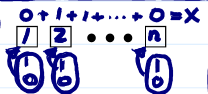
\includegraphics{image/binomail_dist.png}
\end{figure*}

二项分布的特征:
\begin{description}
    \item[参数] $p \in [0,1], n \in \mathbb{N}_+$
    \item[概率质量函数] $p(x)=\begin{cases}
                \binom{n}{x} p^x (1-p)^{n-x} & x \in \mathbb{N}^n \\
                0                            & \text{其他}
            \end{cases}$
    \item[矩母函数] $M(t)=(p e^t + 1-p)^n$,求解方法有:
        \begin{itemize}
            \item \underline{独立变量}之和的矩母函数等于各变量矩母函数之积(参见定理\ref{thm:mgf_sum})
            \item 定义
        \end{itemize}
    \item[均值] $\mu=np$,求解方法有:
        \begin{itemize}
            \item 定义(下述凑一法)
            \item 矩母函数在$t=0$的一阶导
            \item 变量之和的均值等于各变量均值之和
        \end{itemize}
    \item[方差] $\sigma^2=np(1-p)$,求解方法有:
        \begin{itemize}
            \item 定义(下述凑一法)
            \item 矩母函数在$t=0$的二阶导,$\operatorname{Var}(X)=E(X^2)-(E(X))^2$
            \item \underline{独立变量}之和的方差等于各变量均值之和
        \end{itemize}
    \item[实例] 丢$n$次硬币,$p$代表某一面出现的概率,出现此面的次数
\end{description}

\begin{note}
    求解二项分布的均值时,可通过将其凑成概率质量函数之和(为1)的形式:
    \begin{align*}
        E(X) & =\sum_{i=1}^n x \binom{n}{x} p^x (1-p)^{n-x}                 \\
             & = np \sum_{i=1}^n \binom{n-1}{x-1} p^{x-1} (1-p)^{n-1-(x-1)} \\
             & =np
    \end{align*}
    此称为凑一法(sum to one, STO)。同理,求方差时也可使用:
    \begin{align*}
        E(X(X-1))             & =\sum_{i=1}^n x(x-1) \binom{n}{x} p^x (1-p)^{n-x}                   \\
                              & = n(n-1)p^2 \sum_{i=1}^n \binom{n-2}{x-2} p^{x-2} (1-p)^{n-1-(x-1)} \\
                              & =n(n-1)p^2                                                          \\
        \operatorname{Var}(X) & =  E(X(X-1)) + E(X) - (E(X))^2                                      \\
                              & = n(n-1)p^2 + np -n^2 p^2                                           \\
                              & =np(1-p)
    \end{align*}
\end{note}

\begin{proposition}
    二项分布之和仍是二项分布。若$X_1+\cdots+X_k$独立且$X_i \sim B(n_i,p)$,则$Y=X_1+\cdots+X_k  \sim B(n_1+\cdots+n_k,p )$
\end{proposition}

\subsection{几何分布}

\begin{definition}
    若进行无限次独立的Bernouli实验,则第一次出现“1”的实验次数遵循\textbf{几何分布}(geometric distribution),记为$X \sim G(p)$。
\end{definition}

\begin{figure*}[h]
    \centering
    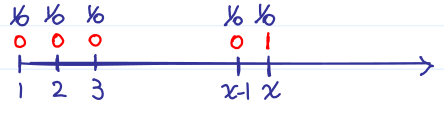
\includegraphics{image/geometric_dist_intu.png}
\end{figure*}

几何分布的特征:
\begin{description}
    \item[参数] $p \in [0,1]$
    \item[概率质量函数] $p(x)=\begin{cases}
                (1-p)^{x-1} p & x \in \mathbb{N}_+ \\
                0             & \text{其他}
            \end{cases}$
    \item[矩母函数] $M(t)=\frac{p e^t}{1-(1-p)e^t}, t<-\ln (1-p)$,求解方法有:
        \begin{itemize}
            \item \underline{独立变量}之和的矩母函数等于各变量矩母函数之积(参见定理\ref{thm:mgf_sum})
            \item 定义
        \end{itemize}
    \item[均值] $\mu=\frac{1}{p}$,求解方法有:
        \begin{itemize}
            \item $E(X)=\sum_{k=1}^{\infty}P(X\ge k)$
            \item 矩母函数在$t=0$的一阶导
            \item 定义(下述微分法)
        \end{itemize}
    \item[方差] $\sigma^2=\frac{1-p}{p^2}$,求解方法有:
        \begin{itemize}
            \item 定义(下述微分法)
            \item 矩母函数在$t=0$的二阶导,$\operatorname{Var}(X)=E(X^2)-(E(X))^2$
        \end{itemize}
    \item[实例] 买彩票时,中奖所需购买张数。
\end{description}

\begin{note}
    微分法求解几何分布均值:
    \begin{align*}
        E(X) & =p\sum_{k=1}^{\infty}k q^{k-1}=p\frac{d}{d q}\sum_{k=1}^{\infty} q^{k} \\
             & =p\frac{d}{d q} \frac{q}{1-q} =\frac{p}{(1-p)^{2}}                     \\
             & =\frac{1}{p}                                                           \\
    \end{align*}
    微分法求解几何分布方差:
    \begin{align*}
        E(X(X-1))             & =p\sum_{k=1}^{\infty}k(k-1) q^{k-1}=p\frac{d}{d q}\sum_{k=1}^{\infty} q^{k} \\
                              & =p\frac{d^2}{d q^2} \frac{q}{1-q} =\frac{2p}{(1-q)^{3}}                     \\
                              & =\frac{2}{p^2}                                                              \\
        \operatorname{Var}(X) & =  E(X(X-1)) + E(X) - (E(X))^2                                              \\
                              & = \frac{2}{p^2} + \frac{1}{p} -\frac{1}{p^2} p^2                            \\
                              & = \frac{1-p}{p^2}
    \end{align*}
\end{note}

\begin{proposition}
    离散分布中有且只有几何分布具备无记忆性:
    \[ P\left\{ X=s+t|X>t \right\} =P\left\{ X=s \right\} ,\quad \forall s>0,t>0\]
\end{proposition}

\begin{proof}
    %TODO 李p135
\end{proof}

\subsection{负二项分布}

\begin{definition}
    若进行无限次独立的Bernouli实验,则第$r$次出现“1”的实验次数遵循\textbf{负二项分布}(negative binomial distribution),记为$X \sim NB(r,p)$。
\end{definition}

\begin{figure*}[h]
    \centering
    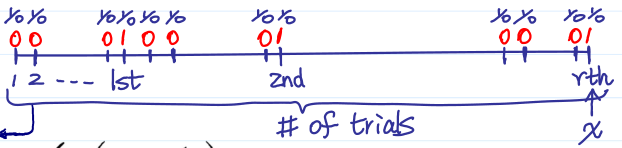
\includegraphics{image/NB_dist_intu.png}
\end{figure*}

负二项分布的特征:
\begin{description}
    \item[参数] $p \in [0,1]$
    \item[概率质量函数] $p(x)=\begin{cases}
                \binom{x-1}{r-1}p^r (1-p)^{x-r} p & x \in \mathbb{N}_r \\
                0                                 & \text{其他}
            \end{cases}$
    \item[矩母函数] $M(t)=\frac{p^r e^{rt}}{(1-(1-p)e^t)^r}, t<-\ln (1-p)$,求解方法有:
        \begin{itemize}
            \item \underline{独立变量}之和的矩母函数等于各变量矩母函数之积(参见定理\ref{thm:mgf_sum})
            \item 定义凑一法
            \item 利用公式$\sum_{x=0}^{\infty}\binom{n+x-1}{x}t^x=\frac{1}{(1-t)^n},-1<t<1$
        \end{itemize}
    \item[均值] $\mu=\frac{r}{p}$,求解方法有:
        \begin{itemize}
            \item 定义凑一法
            \item 矩母函数在$t=0$的一阶导
            \item 独立几何分布之和(定理\ref{prop:sum_of_geo})
        \end{itemize}
    \item[方差] $\sigma^2=\frac{r(1-p)}{p^2}$,求解方法有:
        \begin{itemize}
            \item 定义(凑一法)
            \item 矩母函数在$t=0$的二阶导,$\operatorname{Var}(X)=E(X^2)-(E(X))^2$
            \item 独立几何分布之和(定理\ref{prop:sum_of_geo})
        \end{itemize}
    \item[实例] 买彩票时,中奖$r$次所需购买张数。
\end{description}

\begin{proposition}\label{prop:sum_of_geo}
    几何分布之和是负二项分布。若$X_1+\cdots+X_r$独立且$X_i \sim G(p)$,则$Y=X_1+\cdots+X_r  \sim NB(r,p)$
\end{proposition}

\begin{proof}
    %TODO 
\end{proof}

\begin{proposition}
    负二项分布之和仍是负二项分布。若$X_1+\cdots+X_k$独立且$X_i \sim NB(r_i,p)$,则$Y=X_1+\cdots+X_k  \sim B(r_1+\cdots+r_k,p )$
\end{proposition}

\begin{proof}
    %TODO 
\end{proof}

\subsection{多项分布}

\begin{definition}[多项分布]
    若进行$n$次独立的实验,每次实验有$r$种结果,每种结果对于概率分别为$p_1,\cdots ,p_r$。令$X_i$代表得出结果$i$的次数,则随机向量$\mathbf{X}=(X_1,\cdots ,X_r)$遵循\textbf{多项分布}(multinomial distribution),记为$\mathbf{X} \sim Multinomial(n,p_1,\cdots ,p_r)$。
\end{definition}

多项分布的特征:
\begin{description}
    \item[参数] $p_i \in [0,1], \sum_{i=1}^r p_i=1$
    \item[概率质量函数] $p(x)=\begin{cases}
                \binom{n}{x_1 \cdots x_r} p_1^{x_1}\cdots p_r^{x_r} & x \in \mathbb{N}^n \& \sum_{i=1}^r x_i=n \\
                0                                                   & \text{其他}
            \end{cases}$
    \item[矩母函数] $M(t_1,\cdots ,t_r)=(p_1 e^{t_1} +\cdots + p_r e^{t_r})^n$,求解方法有:
        \begin{itemize}
            \item 利用公式
            \item 凑一法
        \end{itemize}
    \item[边缘分布] $X_i \sim B(n,p_i)$
    \item[均值] $E(X_i)=np_i$
    \item[方差] $\operatorname{Var}(X_i)=np_i(1-p_i)$
    \item[协方差] $\operatorname{Cov}(X_i,X_j)=-p_i p_j$,求解方法有:
        \begin{itemize}
            \item 矩母函数求解$E(X_i X_j)$
            \item 凑一法求解$E(X_i X_j)$
        \end{itemize}
    \item[实例]
\end{description}

\begin{remark}
    多项分布是二项分布的泛化。
\end{remark}

\subsection{泊松分布}

\begin{theorem}[Poisson逼近]\label{thm:Poisson_theorem}
    \[ \lim_{n p_n \to \lambda} \binom{n}{k} p_n^{k} (1-p_n)^{n-k} = \frac{\lambda^{k}}{k !}e^{-\lambda} \]
\end{theorem}

\begin{proof}
    记$np_n=\lambda_n$,记$p_n=\lambda_n/n$,我们可得
    \begin{align*}
        \binom {n}{k} p_n^k(1-p_n)^{n-k} & = \frac{n(n-1)\cdots(n-k+1)}{k!}\left( \frac{\lambda_n}n \right)^k \left( 1 - \frac{\lambda_n}n \right)^{n-k} \\
                                         & = \frac{\lambda_n^k}{k!}\left( 1 - \frac1n \right)\left( 1 - \frac2n \right) \cdots
        \left( 1 - \frac{k-1}n \right)
        \left( 1 - \frac{\lambda_n}n \right)^{n-k}.
    \end{align*}
    对固定的$k$有
    \begin{align*}
         & \lim_{n\to+\infty}\lambda_n = \lambda ;
         & \lim_{n\to+\infty}\left( 1 - \frac{\lambda_n}n \right)^{n-k} = e^{-\lambda} ;
         & \lim_{n\to+\infty}\left( 1 - \frac{1}{n} \right) \cdots \left( 1 - \frac{k-1}n \right) = 1.
    \end{align*}
    从而
    \[
        \lim_{n\to+\infty} \binom{n}{k} p_n^k(1-p_n)^{n-k}  = \frac{\lambda^k}{k!}e^{-\lambda}
    \]
    对任意的$k$($k=0,1,2,\cdots$)成立
\end{proof}

\begin{definition}[Poisson分布]
    若随机变量$X$的概率分布列满足以下形式:
    \[ P(X = k) = \frac{\lambda^k}{k!}e^{-\lambda},\; k = 0,1,2,\cdots, \]
    则称其遵循\textbf{Poisson分布}记为$X\sim P(\lambda)$.
\end{definition}

\begin{remark}
    由定理\ref{thm:Poisson_theorem}可看出,Poisson分布可作为二项分布的近似。$\lambda$的涵义%TODO
\end{remark}

Poisson分布的特征:
\begin{description}
    \item[参数] $\lambda>0$
    \item[概率质量函数] $p(k)=\begin{cases}
                \frac{\lambda^{k}}{k !}e^{-\lambda} & x \in \mathbb{N}^n \\
                0                                   & \text{其他}
            \end{cases}$
    \item[矩母函数] $M(t)=e^{\lambda (e^t -1)}$,求解方法有:
        \begin{itemize}
            \item 利用公式
            \item 凑一法
        \end{itemize}
    \item[均值] $\mu=\lambda$
    \item[方差] $\sigma^2=\lambda$
    \item[实例] 公共汽车站来到的乘客数
\end{description}

\begin{proposition}
    Poisson分布之和仍是Poisson项分布。若$X_1+\cdots+X_k$独立且$X_i \sim P(\lambda_i)$,则$Y=X_1+\cdots+X_k  \sim P(\lambda_1+\cdots+\lambda_k)$
\end{proposition}

\begin{proof}
    %TODO 
\end{proof}

\begin{lemma}\label{lem:Cauchy_lemma}
    若$f(x)$是连续函数(或单调函数),且对一切$x,y$(或一切$x,y\ge 0$)成立:
    \[ f(x)f(y)=f(x+y) \]
    则$f(x)$为\textbf{指数函数}。
\end{lemma}

\begin{proof}
    \begin{align*}
        \because   & f(1)=[f(\frac{1}{n})]^n                           \\
        \text{且}  & a=f(1)=[f(\frac{1}{2})]^2\ge 0                    \\
        \therefore & f(\frac{1}{n})=a^{\frac{1}{n}}                    \\
        \therefore & f(\frac{m}{n})=[f(\frac{1}{n})]^m=a^{\frac{m}{n}}
    \end{align*}
    即此命题对一切有理数成立。又实数具有连续性,故此命题对一切实数成立。
\end{proof}

\begin{definition}[泊松过程]
    若某一随机过程满足以下特征,则称其为\textbf{泊松过程}:
    \begin{description}
        \item[平稳性] 随机事件$A$在$[t_0, t_0 + t)$中的发生次数数只与时间间隔长度$t$有关而与时间起点$t_0$无关。以$P_k(t)$记在长度为$t$的时间区间中发生$K$次事件$A$的概率。
        \item[独立增量性] 在$[t_0, t_0 + t)$中发生$K$次事件$A$的概率与时刻$t_0$以前发生的事件独立。
        \item[普通性] 在充分小的时间间隔中,最多发生一次事件$A$。即,若记$\psi(t)=\sum_{k=2}^{\infty}P_k(t)=1-P_0(t)-P_1(t)$,则有$\lim_{t \to 0}\psi(t)/t=0$
    \end{description}
\end{definition}

对$\Delta t>O$,考虑$[O,t+\Delta t)$中发生$K$次事件$A$的概率$P_k(t+\Delta t)$,由独立增量性及全概率公式可得:
\[ P_k(t+\Delta t)=P_k(t)P_0(\Delta r) + P_{k-1}P_1(\Delta t)+ \cdots +P_0(t)P_k(\Delta t) ,k\ge 0\]
(对$n\ge 1$ ,假定$P_{-n}(t)=0$)

特别地
\[ P_0(t+\Delta t)=P_0(t)P_0(\Delta t) \]
由引理\ref{lem:Cauchy_lemma}知
\[ P_0(t)=a^{t}, a\ge 0 \]
若$a=O$,则$P_0(t) \equiv 0$,说明在不管怎么短的时间间隔内事件$A$都发生,因此在有限时间间隔中将发生无穷多个次事件$A$,这种情形不在我们的考虑之列。此外,因$P_0(t)$是概率,故应有$a\ge 1$,而当$a=1$时,$P_0(t) \equiv 1$,表明事件$A$永不发生,也不是我们感兴趣的情形,所以应有 $0<a<1$,从而存在$\lambda>0$,使
\[ P_0(t)=e^{-\lambda t} \]
因此当$\Delta t \to 0$时,有
\begin{align*}
    P_{0}(\Delta t)                                & =\ee^{-\lambda \Delta t}=1-\lambda \Delta t+o(\Delta t)                  \\
    P_{1}(\Delta t)                                & =1-P_{0}(\Delta t)-\psi(\Delta t)=\lambda \Delta t+o(\Delta t)           \\
    \sum_{l=2}^{\infty} P_{k-l}(t) P_{l}(\Delta t) & \leqslant \sum_{l=2}^{\infty} P_{l}(\Delta t)=\psi(\Delta t)=o(\Delta t) \\
\end{align*}
所以:
\[ P_k(t+\Delta t)=P_k(t)(1-\lambda \Delta t) + P_{k-1}\lambda \Delta t+ o(\Delta t) ,k\ge 1\]
因此:
\[ P'_k(t)= \frac{P_k(t+\Delta t)-P_k(t)}{\Delta t} = \lambda[P_{k-1}-P_k(t)] \]

由于$P_0(t)=\ee^{-\lambda t}$,故有$P'_1(t)=\lambda[\ee^{-\lambda t}-P_1(t)]$,可解得$P_0(t)=\lambda t \ee^{-\lambda t}$,依次可递推可解得:
\[ P_k(t)=\frac{(\lambda t)^k}{k!}\ee^{-\lambda t}, k \in \mathbb{N}\]
正是参数为$\lambda t$的泊松分布。

\subsection{超几何分布}

\begin{definition}
    设有$N$个产品,其中有$M$个不合格品.若从中不放回地随机抽取$n$个,则其中含有的不合格品的个数$X$服从超几何分布,记为$X\sim h(n,N,M)$.
    \begin{equation}\label{eq2.4.6}
        P(X = k) = \frac{\binom Mk \binom{N-M}{n-k}} {\binom Nn},\; k = 0,1,\cdots,r,
    \end{equation}
    其中
\end{definition}

超几何分布的特征:
\begin{description}
    \item[参数] $r=\min\{M,n\}$,且$M\le N,n\le N,n,N,M$均为正整数.
    \item[概率质量函数] $p(k)=\begin{cases}
                \frac{\binom Mk \binom{N-M}{n-k}} {\binom Nn}  k = 0,1,\cdots,r \\
                0 & \text{其他}
            \end{cases}$
    \item[矩母函数] 存在,但没有简单的表达
    \item[均值] $\mu=\frac{rn}{n+m}$
    \item[方差] $\sigma^2=\frac{rnm(n+m-r)}{(n+m)^2(n+m-1)}$
    \item[实例] 从一个有限总体中进行不放回抽样
\end{description}

\begin{remark}
    若$m,n \to \infty$时有$p_{m,n}=\frac{n}{m+n} \to p$,则超几何分布可近似为二项分布。
    $\frac{\binom {M}{k} \binom{N-M}{n-k}} {\binom {N}{n}}
        \cong \binom{n}{k}p^k(1-p)^{n-k}$
\end{remark}

\section{连续分布}

\subsection{均匀分布}

\begin{definition}
    若随机变量$X$在$[a,b]$中任一区域的概率与其测度成正比,则称$X$服从区间$(a,b)$上的\textbf{均匀分布}(Uniform distribution),记作$X\sim U(a,b)$。
\end{definition}

\begin{figure}[!ht]
    \centering
    \subfloat[密度函数$p(x)$]{
        \begin{tikzpicture}[semithick,>=stealth,samples=100,scale=2.5]
            \draw[->](0,0)node[below left]{$O$}--(1.7,0)node[below]{$x$};
            \draw[->](0,0)--(0,1.2)node[right]{$p(x)$};
            \draw[thick](0.3,0.6)--(1.3,0.6);\node[left]at(0,0.6){$\frac1{b-a}$};
            \draw[dashed](0.3,0.6)--(0.3,0)node[below]{$a$}
            (1.3,0.6)--(1.3,0)node[below]{$b$};
        \end{tikzpicture}
    }
    \subfloat[分布函数$F(x)$]{
        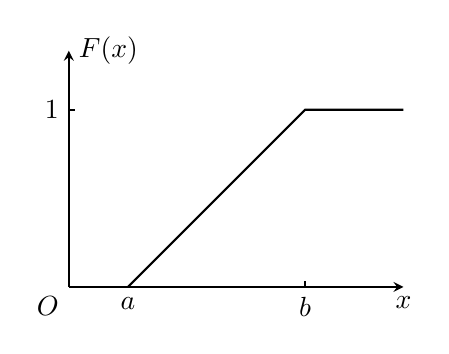
\begin{tikzpicture}[semithick,>=stealth,samples=100,scale=2.5]
            \draw[->](0,0)node[below left]{$O$}--(1.7,0)node[below]{$x$};
            \draw[->](0,0)--(0,1.2)node[right]{$F(x)$};
            \draw[thick](0.3,0)node[below]{$a$}--(1.2,0.9)--(1.7,0.9);
            \draw(1.2,0)node[below]{$b$}--(1.2,0.03);
            \draw(0,0.9)node[left]{$1$}--(0.03,0.9);
        \end{tikzpicture}
    }
    \caption{$(a,b)$上的均匀分布}\label{fig:2.5.3}
\end{figure}

均匀分布的特征:
\begin{description}
    \item[参数] $a<b , \quad a,b \in \mathbb{R} $
    \item[概率质量函数] $p(x)=\begin{cases}
                \frac1{b-a}, & a < x < b   \\
                0            & \text{其他}
            \end{cases}$
    \item[分布函数]  $ F(x) = \begin{cases}
                0,               & x < a ;      \\
                \frac{x-a}{b-a}, & a \le x < b; \\
                1,               & x \ge b.
            \end{cases}$
    \item[矩母函数] $M(t)=\frac{e^{bt}-e^{at}}{t(b-a)} , \quad t \in \mathbb{R}$
    \item[均值] $\mu=\frac{a+b}{2}$
    \item[方差] $\sigma^2=\frac{(b-a)^2}{12}$
\end{description}

\begin{remark}
    常利用$U(0,1)$生成特定分布的伪随机数(参见定理\ref{thm:pseudo_random_generation})
\end{remark}

\subsection{指数分布}

\begin{definition}
    若随机变量X的密度函数(见图 \ref{fig2.5.4})为
    \[ p(x) = \begin{cases}
            \lambda e^{-\lambda x}, & x \ge 0; \\
            0,                      & x < 0,
        \end{cases} \]
    则称$X$服从\textbf{指数分布},记作$X\sim Exp(\lambda)$,其中参数$\lambda>0$. 指数分布的分布函数为
    \[ F(x) = \begin{cases}
            1 - e^{-\lambda x}, & x \ge 0; \\
            0,                  & x < 0.
        \end{cases}\]
\end{definition}

\begin{figure}[!ht]
    \centering
    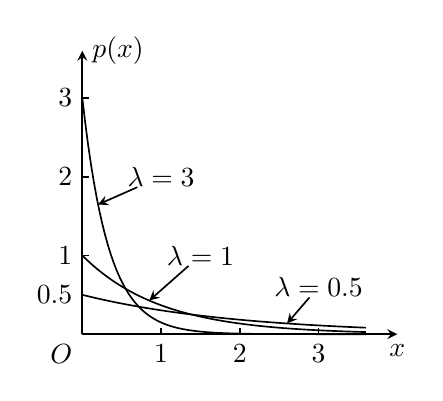
\begin{tikzpicture}[semithick,>=stealth,samples=100]
        \draw[->](0,0)node[below left]{$O$}--(4,0)node[below]{$x$};
        \draw[->](0,0)--(0,3.6)node[right]{$p(x)$};
        \foreach \x in{1,2,3}
        \draw(\x,0)node[below]{$\x$}--(\x,0.08)(0,\x)node[left]{$\x$}--(0.08,\x);
        \draw[domain=0:3.6]plot(\x,{e^(-\x)});
        \draw[domain=0:3.6](0,0.5)node[left]{$0.5$}--plot(\x,{0.5*e^(-0.5*\x)});
        \draw[domain=0:3.6]plot(\x,{3*e^(-3*\x)});
        \node[inner sep=0pt](a)at(1,2){$\lambda=3$};
        \node[inner sep=0pt](b)at(1.5,1){$\lambda=1$};
        \node[inner sep=0pt](c)at(3,0.6){$\lambda=0.5$};
        \draw[->](a)--(0.2,{3*e^(-3*0.2)});
        \draw[->](b)--(0.85,{e^(-0.85)});
        \draw[->](c)--(2.6,{0.5*e^(-0.5*2.6)});
    \end{tikzpicture}
    \caption{参数为$\lambda$的指数分布密度函数}\label{fig2.5.4}
\end{figure}

指数分布的特征:
\begin{description}
    \item[矩母函数] $M(t)=\frac{\lambda}{\lambda-t} , \quad t < \lambda$
    \item[均值] $\mu=\frac{1}{\lambda}$
    \item[方差] $\sigma^2=\frac{1}{\lambda^{2}}$
    \item[实例] 物品使用寿命,等待时间
\end{description}

\begin{remark}
    有其均值可看出,对于等待时间模型,$\frac{1}{\lambda}$代表平均等待时间,即(时间/次);$\lambda$代表平均发生频率,即(次/时间)。
\end{remark}

\begin{theorem}[指数分布的无记忆性]
    连续分布中有且只有指数分布具备无记忆性:
    \[ P(X > s + t| X > s) = P( X > t) ,\quad \forall s>0,t>0\]
\end{theorem}

\begin{proof}
    %TODO 李p138
\end{proof}

\begin{proposition}
    如果某设备在任何长为$t$的时间$[0,t]$内发生故障的次数$N9t)$服从参数为$\lambda t$的泊松分布,则相继两次故障之间的时间间隔$T$服从参数为$\lambda$的指数分布.
\end{proposition}

\begin{proof}
    设$N(t)\sim P(\lambda t)$,即
    \[
        P\big( N(t) = k \big) = \frac{(\lambda t)^k}{k!} e^{-\lambda t},\quad k=0,1,\cdots.
    \]

    注意到两次故障之间的时间间隔$T$是非负随机变量,且事件$\{T\ge t\}$说明此设备在$[0,t]$内没有发生故障,即$\{T\ge t\}=\{N(t)=0\}$,由此我们得

    当$t<0$时,有$F_T(t)=P(T\le t)=0$;

    当$t\ge0$时,有
    \[
        F_T(t) = P(T\le t) = 1 - P(T>t) = 1 -P\big( N(t)=0 \big) = 1 - e^{-\lambda t},
    \]
    所以$T\sim Exp(\lambda)$,相继两次故障之间的时间间隔$T$服从参数为$\lambda$的指数分布.
\end{proof}

\subsection{伽马分布}

\begin{definition}
    若随机变量$X$的密度函数为
    \[ p(x) = \begin{cases}
            \frac{\lambda^\alpha}{\Gamma(\alpha)}x^{\alpha-1}
            \ee^{-\lambda x}, & x\ge 0 ; \\
            0,                & x < 0,
        \end{cases} \]
    则称$X$服从\textbf{伽玛分布},记作$X\sim \Gamma(\alpha,\lambda)$,其中$\alpha>0$为形状参数,$\lambda>0$为尺度参数.
\end{definition}



图 \ref{fig2.5.5} 给出若于条$\lambda$固定、$\alpha$不同的伽玛密度函数曲线,从图中可以看出:

\begin{itemize}
    \item $0<\alpha<1$时,$p(x)$是严格下降函数,且在$x=0$处有奇异点;
    \item $\alpha=1$时,$p(x)$是严格下降函数,且在$x=0$处$p(0)=\lambda$;
    \item $1<\alpha\le2$,$p(x)$是单峰函数,向上凸、后下凸;
    \item $2<\alpha$时,$p(x)$是单峰函数,先下凸、中间上凸、后下凸. 且$\alpha$越大,$p(x)$越近似于正态分布.
\end{itemize}

\begin{figure}[!ht]
    \centering
    \subfloat{
        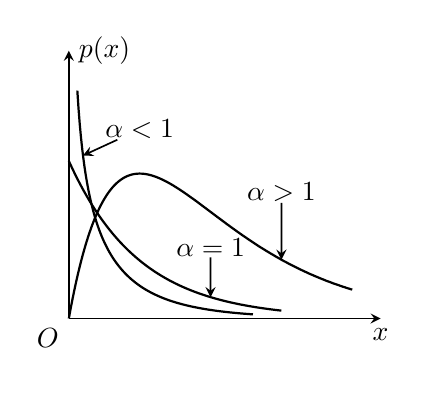
\begin{tikzpicture}[semithick,>=stealth,samples=150,yscale=2,xscale=0.9]
            \draw[->](0,0)node[below left]{$O$}--(4.4,0)node[below]{$x$};
            \draw[->](0,0)--(0,1.7)node[right]{$p(x)$};
            \draw[thick,domain=0.12:2.6]plot(\x,{e^(-\x)/sqrt(\x)/1.77});
            \draw[thick,domain=0:3]plot(\x,{e^(-\x)});
            \draw[thick,domain=0:4]plot(\x,{2.5*(\x)*e^(-\x)});
            \node[inner sep=0pt](a)at(2,0.45){$\alpha=1$};
            \node[inner sep=0pt](b)at(1,1.2){$\alpha<1$};
            \node[inner sep=0pt](c)at(3,0.8){$\alpha>1$};
            \draw[->](a)--(2,{e^(-2)});
            \draw[->](b)--(0.2,{e^(-0.2)/sqrt(0.2)/1.77});
            \draw[->](c)--(3,{2.5*(3)*e^(-3)});
            \node[below]at(1,0){\phantom{$\frac{\alpha-1}\lambda$}};
        \end{tikzpicture}
    }
    \subfloat{
        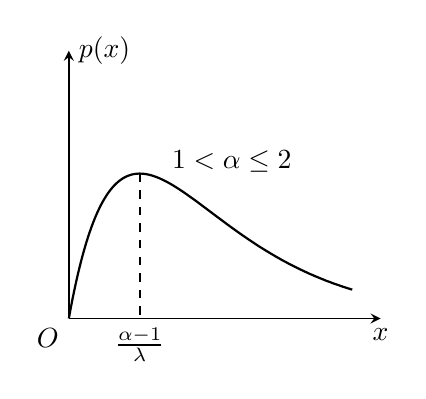
\begin{tikzpicture}[semithick,>=stealth,samples=150,yscale=2,xscale=0.9]
            \draw[->](0,0)node[below left]{$O$}--(4.4,0)node[below]{$x$};
            \draw[->](0,0)--(0,1.7)node[right]{$p(x)$};
            \draw[thick,domain=0:4]plot(\x,{2.5*(\x)*e^(-\x)});
            \draw[dashed](1,{2.5*e^(-1)})--(1,0)node[below]{$\frac{\alpha-1}\lambda$};
            \node at(2.3,1){$1<\alpha\leq2$};
        \end{tikzpicture}
    }
    \subfloat{
        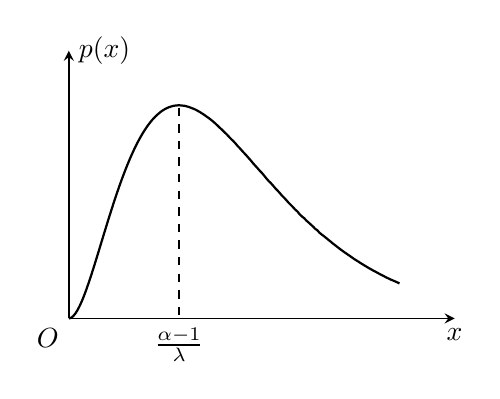
\begin{tikzpicture}[semithick,>=stealth,samples=150,yscale=2,xscale=0.7]
            \draw[->](0,0)node[below left]{$O$}--(7,0)node[below]{$x$};
            \draw[->](0,0)--(0,1.7)node[right]{$p(x)$};
            \draw[thick,domain=0:6]plot(\x,{2.5*(\x)^2*e^(-\x)});
            \draw[dashed](2,{1.5*2^2*e^(-1.5)})--(2,0)node[below]{$\frac{\alpha-1}\lambda$};
        \end{tikzpicture}
    }
    \caption{$\lambda$固定、不同$\alpha$的伽玛密度曲线}\label{fig2.5.5}
\end{figure}

Gamma分布的特征:
\begin{description}
    \item[矩母函数] $M(t)=(\frac{\lambda}{\lambda-t})^{\alpha} , \quad t<\lambda$
    \item[均值] $\mu=\frac{\alpha}{\lambda}$
    \item[方差] $\sigma^2=\frac{\alpha}{\lambda^{2}}$
\end{description}

Gamma函数$\Gamma(\alpha)=\int_0^{\infty}y^{\alpha-1}\ee^{-y}dy$的特征:
\begin{itemize}
    \item $\Gamma(1)=1$
    \item $\Gamma(\frac{1}{2})=\sqrt{\pi}$
    \item $\Gamma(\alpha)=(\alpha-1)\Gamma(\alpha-1)$
    \item $\Gamma(n)=(n-1)!,\quad n \in \mathbb{Z}$
    \item $\Gamma(\frac{\alpha}{2})=\frac{\sqrt{\pi}(\alpha-1)!}{2^{\alpha-1}(\frac{\alpha-1}{2})!}, \quad \alpha=2k+1,k \in \mathbb{N}$
\end{itemize}

\begin{proposition}\label{prop:sum_of_Gamma}
    $\Gamma$分布是指数分布的泛化,即$\Gamma(1,\lambda)=E(\lambda)$。进一步有:若随机变量$X_1,\cdots ,X_k, \operatorname{i.i.d.} \sim E(\lambda)$,则$Y=X_1+\cdots+X_k  \sim \Gamma(k,\lambda)$。更进一步有:若随机变量$X_1',\cdots ,X_k', \operatorname{i.i.d.} \sim \Gamma(\alpha_i,\lambda)$,则$Y'=X_1'+\cdots+X_k'  \sim \Gamma(\alpha_1+\cdots +\alpha_k,\lambda)$。
\end{proposition}

\begin{proof}
    \begin{align*}
        M_Y(t)    & =\prod_{i=1}^k M_{X_i}(t_i)=\prod_{i=1}^k \frac{\lambda}{\lambda-t}=(\frac{\lambda}{\lambda-t})^{k}                                       \\
        M_{Y'}(t) & =\prod_{i=1}^k M_{X_i'}(t_i)=\prod_{i=1}^k (\frac{\lambda}{\lambda-t})^{\alpha_i}=(\frac{\lambda}{\lambda-t})^{\alpha_1+\cdots +\alpha_k}
    \end{align*}
\end{proof}

\begin{proposition}
    若令随机变量$X \sim \Gamma(\alpha,\lambda)$,则$cX \sim \Gamma(\alpha,\frac{\lambda}{c}), \quad c>0$
\end{proposition}

\begin{proof}
    \[ M_{c X}(t) = M_X(c t) =(\frac{\lambda}{\lambda-c t})^{\alpha}=(\frac{\frac{\lambda}{c}}{\frac{\lambda}{c}-t})^{\alpha}\]
\end{proof}

\begin{proposition}
    若令随机变量$X \sim \Gamma(\alpha,\lambda)$,则$\mu_k=\frac{\Gamma(\alpha+k)}{\lambda^{k}\Gamma(\alpha)}, \quad 0<k$,且则$\mu_{-k}=\frac{\lambda^{k}\Gamma(\alpha-k)}{\Gamma(\alpha)}, \quad 0<k<\alpha$
\end{proposition}

\begin{proof}
    \begin{align*}
        \mu_k=M_X^{(k)}(0)     & =\frac{1}{\lambda^{k}}\alpha(\alpha+1)\cdots(\alpha+k-1) =\frac{\Gamma(\alpha+k)}{\lambda^{k}\Gamma(\alpha)} \\
        \mu_{-k}=M_X^{(-k)}(0) & =\lambda^{k}\frac{1}{\alpha-1}\cdots\frac{1}{\alpha-k} =\frac{\lambda^{k}\Gamma(\alpha-k)}{\Gamma(\alpha)}
    \end{align*}
\end{proof}



\begin{proposition}
    %TODO 指数分布、伽马分布与泊松分布间的联系
\end{proposition}

\subsection{贝塔分布}

\begin{definition}
    称以下函数
    \[ \beta(a,b) = \int_0^1 x^{a-1}(1-x)^{b-1}\dd x \]
    为\textbf{贝塔函数},其中参数$a>0,b>0$.
\end{definition}

\begin{proposition}
    贝塔函数具有如下性质:
    \begin{itemize}
        \item $\beta(a,b)=\beta(b,a)$
        \item $\beta(a,b) = \frac{\Gamma(a)\Gamma(b)}{\Gamma(a+b)}$
    \end{itemize}
\end{proposition}

\begin{proof}
    在贝塔函数的积分中令$y=1-x$,即得
    \[ \beta(a,b) = \int_1^0(1-y)^{a-1}y^{b-1}(-\dd y) = \int_0^1 (1-y)^{a-1}y^{b-1}\dd y = \beta(b,a) \]
    由伽玛函数的定义知
    \[ \Gamma(a) \Gamma(b) = \int_0^{+\infty}\int_0^{+\infty}x^{a-1}y^{b-1}  \ee^{-(x+y)} \dd x \dd y \]
    作变量变换$x=uv,y=u(1-v)$,其雅可比行列式$J=-u$,故
    \begin{align*}
        \Gamma(a)\Gamma(b) & = \int_0^{+\infty}\int_0^1(uv)^{a-1}[u(1-v)]^{b-1}
        \ee^{-u}u \dd u \dd v                                                                    \\
                           & = \int_0^{+\infty}u^{a+b-1}\ee^{-u} \int_0^1v^{a-1}(1-v)^{b-1}\dd v
        = \Gamma(a+b)                                                                            \\beta(a,b),
    \end{align*}
\end{proof}

\begin{definition}
    若随机变量$X$的密度函数为
    \[ p(x) = \begin{cases}
            \frac{\Gamma(a+b)}{\Gamma(a)\Gamma(b)}
            x^{a-1}(1-x)^{b-1}, & 0 < x < 1;   \\
            0,                  & \text{其他},
        \end{cases} \]
    则称$X$服从\textbf{贝塔分布},记作$X\sim Be(a,b)$,其中$a>0,b>0$都是形状参数.
\end{definition}

\begin{figure}
    \centering
    \subfloat{
        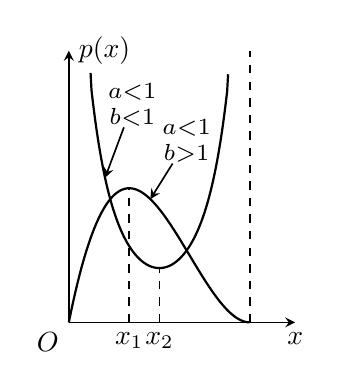
\begin{tikzpicture}[semithick,>=stealth,samples=150,scale=2.3]
            \draw[->](0,0)node[below left]{$O$}--(1.25,0)node[below]{$x$};
            \draw[->](0,0)--(0,1.5)node[right]{$p(x)$};
            \draw[thick,domain=0:1] plot(\x,{5*(\x)*(1-\x)^2});
            \draw[thick,domain=0.12:0.88] plot(\x,{(\x)^(-1/2)*(1-\x)^(-1/2)-1.7});
            \draw[dashed](1,0)--(1,1.5);
            \node[inner sep=0pt](a)at(0.35,1.2){\scalebox{1.2}{$a<1\atop b<1$}};
            \node[inner sep=0pt](b)at(0.65,1){\scalebox{1.2}{$a<1\atop b>1$}};
            \draw[->](a)--(0.2,{(0.2)^(-1/2)*(1-0.2)^(-1/2)-1.7});
            \draw[->](b)--(0.45,{5*(0.45)*(1-0.45)^2});
            \draw[dashed](1/3,0)node[below]{$x_1$}--(1/3,{5*(1/3)*(1-1/3)^2});
            \draw[dashed](0.5,0)node[below]{$x_2$}--(0.5,{(0.5)^(-1/2)*(1-0.5)^(-1/2)-1.7});
        \end{tikzpicture}
    }
    \subfloat{
        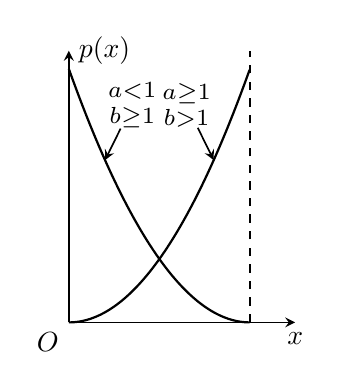
\begin{tikzpicture}[semithick,>=stealth,samples=150,scale=2.3]
            \draw[->](0,0)node[below left]{$O$}--(1.25,0)node[below]{$x$};
            \draw[->](0,0)--(0,1.5)node[right]{$p(x)$};
            \draw[thick,domain=0:1] plot(\x,{1.4*(1-\x)^2});
            \draw[thick,domain=0:1] plot(\x,{1.4*(\x)^2});
            \node[inner sep=0pt](a)at(0.35,1.2){\scalebox{1.2}{$a<1\atop b\geq1$}};
            \node[inner sep=0pt](b)at(0.65,1.2){\scalebox{1.2}{$a\geq1\atop b>1$}};
            \draw[->](a)--(0.2,{1.4*(0.8)^2});
            \draw[->](b)--(0.8,{1.4*0.8^2});
            \draw[dashed](1,0)--(1,1.5);
        \end{tikzpicture}
    }
    \subfloat{
        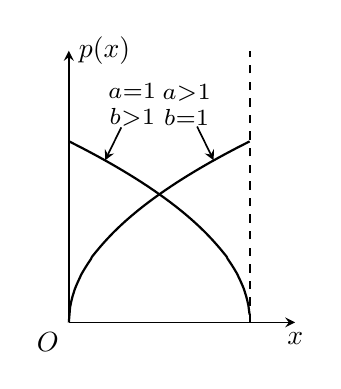
\begin{tikzpicture}[semithick,>=stealth,samples=150,scale=2.3]
            \draw[->](0,0)node[below left]{$O$}--(1.25,0)node[below]{$x$};
            \draw[->](0,0)--(0,1.5)node[right]{$p(x)$};
            \draw[thick,domain=0:1] plot(\x,{1*(1-\x)^(1/2)});
            \draw[thick,domain=0:1] plot(\x,{1*(\x)^(1/2)});
            \node[inner sep=0pt](a)at(0.35,1.2){\scalebox{1.2}{$a=1\atop b>1$}};
            \node[inner sep=0pt](b)at(0.65,1.2){\scalebox{1.2}{$a>1\atop b=1$}};
            \draw[->](a)--(0.2,{1*(0.8)^(1/2)});
            \draw[->](b)--(0.8,{1*0.8^(1/2)});
            \draw[dashed](1,0)--(1,1.5);
        \end{tikzpicture}
    }
    \subfloat{
        \begin{tikzpicture}[semithick,>=stealth,samples=150,scale=2.3]
            \draw[->](0,0)node[below left]{$O$}--(1.25,0)node[below]{$x$};
            \draw[->](0,0)--(0,1.5)node[right]{$p(x)$};
            \draw[thick](0,0.7)--(1,0.7);
            \draw[dashed](1,0)node[below]{$1$}--(1,0.7);
            \node[inner sep=0pt](a)at(0.6,1){\scalebox{1.2}{$a=1\atop b=1$}};
            \draw[->](a)--(0.3,0.7);
        \end{tikzpicture}
    }
    \caption{贝塔密度函数曲线}\label{fig2.5.6}
\end{figure}

从图 \ref{fig2.5.6} 可以看出:
\begin{itemize}
    \item $a<1,b<1$时,$p(x)$是下凸的单峰函数.
    \item $a>1,b>1$时,$p(x)$是上凸的单峰函数.
    \item $a<10,b\ge1$时,$p(x)$是下凸的单调减函数.
    \item $a\ge1,b<1$时,$p(x)$是下凸的单调增函数.
    \item $a=1,b=1$时,$p(x)$是常函数,且$Be(1,1)=U(0,1)$.
\end{itemize}

Beta分布的特征:
\begin{description}
    \item[矩母函数] $M(t)=1+\sum_{k=1}^{\infty}(\prod_{r=0}^{k-1} \frac{a+r}{a+b+r})\frac{t^k}{k!}, \quad t<\lambda$
    \item[均值] $\mu=\frac{a}{a+b}$
    \item[方差] $\sigma^2=\frac{ab}{(a+b+1)(a+b)^{2}}$
\end{description}

\begin{remark}
    \[ \beta(1,1)=U(0,1) \]
\end{remark}

\begin{proposition}
    令独立随机变量$X_1 \sim \Gamma(\alpha_1,\lambda),X_2 \sim  \Gamma(\alpha_2,\lambda)$,则$\frac{X_1}{X_1+X_2} \sim \beta(\alpha_1,\alpha_2)$
\end{proposition}

\begin{proof}
    %TODO 李P182习题38
\end{proof}

\section{正态分布及其导出分布}

\subsection{正态分布}

\begin{definition}
    若随机变量$X$的密度函数为
    \begin{equation}\label{eq2.5.1}
        p(x) = \frac1{\sqrt{2\pi}\sigma} \ee^{-\frac{(x-\mu)^2}{2\sigma^2}},x \in \mathbb{R}
    \end{equation}
    则称$X$服从\textbf{正态分布}(Normal distribution),称$X$为\textbf{正态变量},记作$X\sim N(\mu,\sigma^2)$。其中参数$\mu \in \mathbb{R},\sigma>0$。
\end{definition}

正态分布的密度函数$p(x)$的图形如图 \ref{fig2.5.1}(a)所示,是一条钟形曲线,左右关于$\mu$对称,衰减速度由$\sigma$决定,$\mu\pm\sigma$是该曲线的拐点.

\begin{figure}[!ht]
    \centering
    \subfloat[密度函数$p(x)$]{
        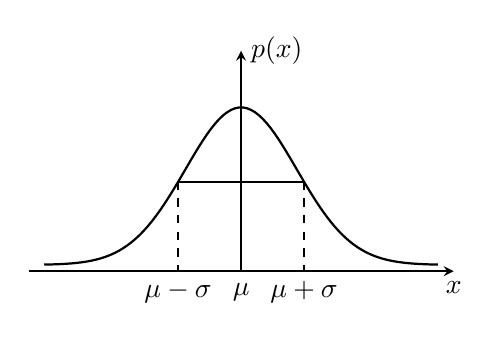
\begin{tikzpicture}[semithick,yscale=2,>=stealth]
            \draw[->](-2.7,0)--(0,0)node[below=1pt]{$\mu$}--(2.7,0)node[below]{$x$};
            \draw[->](0,0)--(0,1.4)node[right]{$p(x)$};
            \draw[samples=100,domain=-2.5:2.5,thick]plot(\x,{e^(-(\x)^2)+0.04});
            \draw[dashed](-0.8,{e^(-0.64)+0.04})--(-0.8,0)node[below]{$\mu-\sigma$}
            (0.8,{e^(-0.64)+0.04})--(0.8,0)node[below]{$\mu+\sigma$};
            \draw(0.8,{e^(-0.64)+0.04})--(-0.8,{e^(-0.64)+0.04});
        \end{tikzpicture}
    }\hspace{1.5cm}
    \subfloat[分布函数$F(x)$]{
        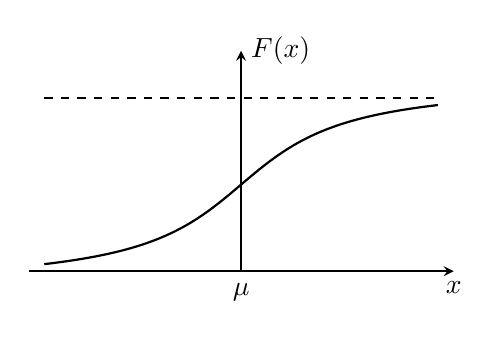
\begin{tikzpicture}[semithick,yscale=2,>=stealth]
            \draw[->](-2.7,0)--(0,0)node[below=1pt]{$\mu$}--(2.7,0)node[below]{$x$};
            \draw[->](0,0)--(0,1.4)node[right]{$F(x)$};
            \draw[samples=100,domain=-2.5:2.5,thick]plot(\x,{(atan(\x))/135+0.55});
            \draw[dashed](-2.5,1.1)--(2.5,1.1);
        \end{tikzpicture}
    }
    \caption{正态分布}\label{fig2.5.1}
\end{figure}

正态分布的特征:
\begin{description}
    \item[矩母函数] $M(t)=\exp (\mu t + \frac{\sigma^2 t^2}{2}), \quad t \in \mathbb{R}$
    \item[均值] $\mu=\mu$
    \item[方差] $\sigma^2=\sigma^2$
\end{description}

\begin{proposition}
    若随机变量$X \sim N(\mu, \sigma^2)$,则其线性变换$a,b \in \mathbb{R},aX + b \sim N(a \mu + b,a^2 \sigma^2)$。特别的,常对正态随机变量作标准化:$\frac{X-\mu}{\sigma} \sim N(0,1)$
\end{proposition}

\begin{proof}
    \[ M_{aX + b}(t)=e^{bt}M_X(a t)=\exp (bt + a \mu t+\frac{a^2 \sigma^2 t^2}{2}) \]
\end{proof}

\begin{proposition}
    若独立随机变量$X_1,\cdots ,X_k$满足$ X_i \sim N(\mu_i,\sigma_i^2)$,则其和$Y=X_1+\cdots +X_k \sim N(\sum_{i=1}^k\mu_i,\sum_{i=1}^k\sigma_i^2)$
\end{proposition}

\begin{proof}
    \[ M_{X_1+\cdots+ X_n} = \prod_{i=1}^n M_{X_i}(t)=\exp (\sum_{i=1}^k\mu_i t + \sum_{i=1}^k \frac{\sigma_i^2 t^2}{2}) \]
\end{proof}

\begin{corollary}
    若随机变量$X_1,\cdots ,X_k \operatorname{i.i.d.} \sim N(\mu,\sigma^2)$,则其平均$\overline{X}=(X_1+\cdots +X_k)/k \sim N(\mu,\frac{\sigma^2}{k})$
\end{corollary}

\begin{theorem}\label{thm:normal_sample_mean_variance}
    若随机变量$X_1,\cdots ,X_k \operatorname{i.i.d} \sim N(\mu,\sigma^2)$,并且定义其样本均值为$\overline{X_n}=\frac{1}{n}\sum_{i=1}^n X_i$,其样本方差为$S_n^2=\frac{1}{n-1}\sum_{i=1}^n (X_i-\overline{X_n})^2$,则有以下关系:
    \begin{enumerate}
        \item $\overline{X_n} \sim N(\mu,\frac{\sigma^2}{n})$,即$\sqrt{n}(\overline{X_n}-\mu)/\sigma \sim N(0,1)$
        \item 随机变量$\overline{X_n}$与随机向量$(X_1-\overline{X_n},\cdots ,X_n-\overline{X_n})$独立
        \item $\overline{X_n},S_n^2$独立
        \item $\frac{(n-1)S_n^2}{\sigma} \sim \chi_n$
        \item $\frac{\sqrt{n}(\overline{X_n}-\mu)}{S_n} \sim t_{n-1}$
    \end{enumerate}
\end{theorem}
\begin{proof}
    %TODO
\end{proof}

\subsection{卡方分布}

\begin{definition}
    设$Z_1,\dotsc,Z_n$独立同分布于标准正态分布$N(0,1)$,则$X=Z_1^2+\dotsc+Z_n^2$的分布称为\textbf{$n$自由度}的\textbf{卡方分布}(Chi-square distribution),记为$X \sim \chi^2_n$.
\end{definition}

卡方分布的特征:
\begin{description}
    \item[参数] $n \in \mathbb{N}_+$
    \item[概率密度函数] $p(x)=\begin{cases}
                \frac{(1/2)^{\frac n2}}{\Gamma(n/2)}y^{\frac n2-1}\ee^{-\frac y2} & y>0         \\
                0                                                                 & \text{其他}
            \end{cases}$
    \item[矩母函数] $M(t)=(\frac{1}{1-2t})^{\frac{n}{2}}$
    \item[均值] $\mu=n$
    \item[方差] $\sigma^2=2n$
    \item[实例]
\end{description}

该密度函数的图像是一个只取非负值的偏态分布,见图~\ref{fig:5.4.1}。
\begin{figure}[!ht]
    \centering
    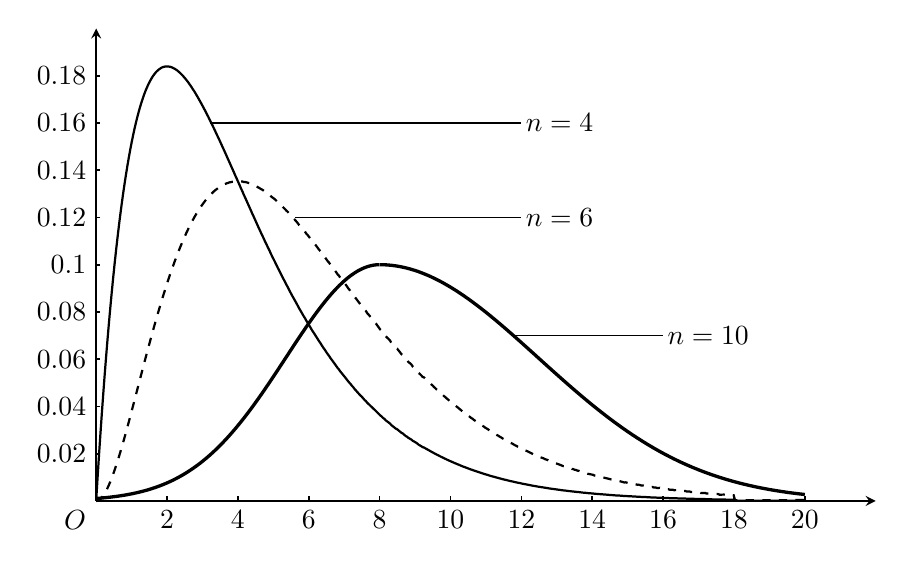
\begin{tikzpicture}[>=stealth,semithick,xscale=0.45,yscale=30,samples=500]
        \draw[->](0,0)node[below left]{$O$}--(22,0);
        \foreach\x in{2,4,...,20}\draw(\x,0.002)--(\x,0)node[below]{\x};
        \draw[->](0,0)--(0,0.2);
        \foreach\x in{0.02,0.04,0.06,0.08,0.1,0.12,0.14,0.16,0.18}\draw(0,\x)node[left]{\x}--(0.12,\x);
        \draw[thick,domain=0:20]plot(\x,{(\x)*e^(-(\x)/2)/4});
        \draw(3.2,0.16)--(12,0.16)node[right=-2pt]{$n=4$};
        \draw[thick,dashed,domain=0:20]plot(\x,{(\x)^2*e^(-(\x)/2)/16});
        \draw[very thick,domain=0:8]plot(\x,{0.1*e^(-(\x-8)^2/14)});
        \draw[very thick,domain=8:20]plot(\x,{0.1*e^(-(\x-8)^2/40)});
        \draw(5.62,0.12)--(12,0.12)node[right=-2pt]{$n=6$};
        \draw(11.8,0.07)--(16,0.07)node[right=-2pt]{$n=10$};
    \end{tikzpicture}
    \caption{$\chi^2(n)$分布的密度函数}\label{fig:5.4.1}
\end{figure}

\begin{proposition}
    若 $X\sim N(0,1)$,则$X^2\sim Ga(1/2,1/2),Y \sim Ga(n/2,1/2)=\chi^2(n)$
\end{proposition}

\begin{proof}
    %TODO \ref{prop:sum_of_Gamma}
\end{proof}

\begin{corollary}
    若随机变量$X_1,\cdots ,X_k, \operatorname{i.i.d.} \sim \chi^2_{n_i}$,则$Y=X_1+\cdots+X_k  \sim \chi^2_{n_1+\cdots +n_k}$。
\end{corollary}

\subsection{F分布}

\begin{definition}{}{}
    设独立随机变量$X_1\sim\chi^2(m),X_2\sim\chi^2(n)$,则称$F=\frac{X_1/m}{X_2/n}$的分布是自由度为$m$与$n$的\textbf{F分布},记为$F\sim F(m,n)$,其中$m$称为\underline{分子自由度},$n$称为\underline{分母自由度}。
\end{definition}

F分布的特征:
\begin{description}
    \item[参数] $m,n \in \mathbb{N}_+$
    \item[概率密度函数]
        \[ f(x)=\frac{\Gamma \left( \frac{m+n}{2} \right) }{\Gamma \left( \frac{m}{2} \right) \Gamma \left( \frac{n}{2} \right)}\left( \frac{m}{n} \right) ^{\frac{m}{2}}x^{\frac{m}{2}-1}\left( 1+\frac{m}{n}x \right) ^{-\frac{m+n}{2}} \]
    \item[矩母函数] 不存在
    \item[均值] $\mu=\frac{n}{n-2}$
    \item[方差] $\sigma^2=\frac{2n^2(m+n-2)}{m(n-2)^2(n-4)}$
    \item[实例]
\end{description}

\begin{figure}
    \centering
    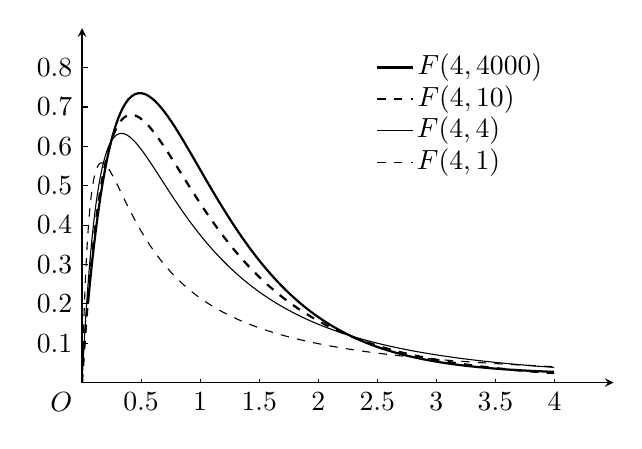
\begin{tikzpicture}[xscale=1.5,yscale=5,>=stealth,domain=0:4,samples=500]
        \draw[->](0,0)node[below left]{$O$}--(4.5,0);\draw[->](0,0)--(0,0.9);
        \foreach \x in{0.5,1,...,4}\draw(\x,0.01)--(\x,0)node[below]{$\x$};
        \foreach \x in{0.1,0.2,0.3,0.4,0.5,0.6,0.7,0.8}\draw(0.05,\x)--(0,\x)node[left]{$\x$};
        \draw[dashed]plot (\x,{12*(\x)/(1+4*(\x))^(5/2)});
        \draw plot (\x,{6*(\x)/(1+\x)^4});
        \draw[thick,dashed]plot (\x,{4.8*(\x)/(1+0.4*(\x))^7});
        \draw[thick,domain=0.05:4]plot (\x,{4*(\x)/(1+0.04*\x)^52+0.02});
        \draw[thick](2.5,.8)--(2.8,.8)node[right=-2pt]{$F(4,4000)$};
        \draw[thick,dashed](2.5,.72)--(2.8,.72)node[right=-2pt]{$F(4,10)$};
        \draw(2.5,.64)--(2.8,.64)node[right=-2pt]{$F(4,4)$};
        \draw[dashed](2.5,.56)--(2.8,.56)node[right=-2pt]{$F(4,1)$};
    \end{tikzpicture}
    \caption{$F$分布的密度函数,是一个只取非负值的偏态分布}\label{fig:5.4.2}
\end{figure}

\begin{proposition}
    $F$分布的密度函数为
\end{proposition}

\begin{proof}
    首先我们导出$Z=\frac{X_1}{X_2}$的密度函数,若记$p_1(x)$和$p_2(x)$分别为$\chi^2(m)$和$\chi^2(n)$的密度函数,根据独立随机变量商的分布的密度函数公式\ref{equ:quotient_of_variable}。$Z$的密度函数为
    \begin{align*}
        p_Z(z) & =\int_0^{=\infty}x_2p_1(zx_2)p_2(x_2)\dd x_2                                                                                                                                       \\
               & =\frac{z^{\frac{m}{2}-1}}{\Gamma \left( \frac{m}{2} \right) \Gamma \left( \frac{n}{2} \right) 2^{\frac{m+n}{2}}}\int_0^{+\infty}x_2^{\frac{m+n}2-1}\ee^{-\frac{x_2}2(1+z)}\dd x_2.
    \end{align*}
    运用变换$u=\frac{x_2}2(1+z)$,可得
    \[p_Z(z)=\frac{z^{\frac{m}{2}-1}\left( 1+z \right) ^{\frac{m+n}{2}}}{\Gamma \left( \frac{m}{2} \right) \Gamma \left( \frac{n}{2} \right)}\int_0^{+\infty}u^{\frac{m+n}2-1}\ee^{-u}\dd u.\]
    最后的定积分为伽马函数$\Gamma\left(\frac{m+n}2\right)$,从而
    \[
        p_Z\left( z \right) =\frac{\Gamma \left( \frac{m+n}{2} \right)}{\Gamma \left( \frac{m}{2} \right) \Gamma \left( \frac{n}{2} \right)}z^{\frac{m}{2}-1}\left( 1+z \right) ^{-\frac{m+n}{2}},\quad z>0.
    \]
    第二步,我们导出$F=\frac nm Z$的密度函数,对$y>0$,有
    \begin{align*}
        p_F\left( y \right) & =p_Z\left( \frac{m}{n}y \right) \cdot \frac{m}{n}                                                                                                                                                                            \\
                            & =\frac{\Gamma \left( \frac{m+n}{2} \right)}{\Gamma \left( \frac{m}{2} \right) \Gamma \left( \frac{n}{2} \right)}\left( \frac{m}{n}y \right) ^{\frac{m}{2}-1}\left( 1+\frac{m}{n}y \right) ^{-\frac{m+n}{2}}\cdot \frac{m}{n} \\
                            & =\frac{\Gamma \left( \frac{m+n}{2} \right) \left( \frac{m}{n} \right) ^{\frac{m}{2}}}{\Gamma \left( \frac{m}{2} \right) \Gamma \left( \frac{n}{2} \right)}y^{\frac{m}{2}-1}\left( 1+\frac{m}{n}y \right) ^{-\frac{m+n}{2}}.
    \end{align*}
\end{proof}

\begin{remark}
    由$F$分布的构造知,若$F\sim F(m,n)$,则有$1/F\sim F(n,m)$
\end{remark}

\subsection{t分布}

\begin{definition}
    设随机变量$Z \sim N(0,1)$与$U \sim\chi^2_n$独立,则称$t=\frac{Z}{\sqrt{U/n}}$的分布为自由度为$n$的\textbf{t分布},记为$t \sim t_n$.
\end{definition}

$t$分布的密度函数的图像是一个关于纵轴对称的分布(图~\ref{fig:5.4.3} ),与标准正态分布的密度函数形状类似,只是峰比标准正态分布低一些,尾部的概率比标准正态分布的大一些.
\begin{figure}
    \centering
    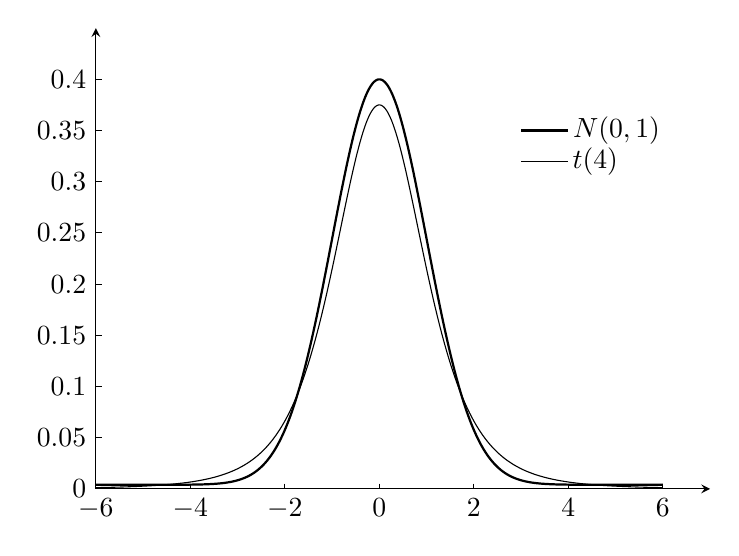
\begin{tikzpicture}[xscale=0.6,yscale=13,>=stealth,domain=-6:6,samples=500]
        \draw[->](-6,0)--(7,0);\draw[->](-6,0)--(-6,0.45);
        \foreach \x in{-6,-4,...,6}\draw(\x,0.005)--(\x,0)node[below]{$\x$};
        \foreach \x in{0,0.05,0.1,0.15,0.2,0.25,0.3,0.35,0.4}\draw(-5.88,\x)--(-6,\x)node[left]{$\x$};
        \draw[thick]plot(\x,{0.396*e^(-(\x)^2/2)+0.004});
        \draw plot(\x,{0.375*(1+(\x)^2/4)^(-5/2)});
        \draw[thick](3,0.35)--(4,0.35)node[right=-2pt]{$N(0,1)$};
        \draw(3,0.32)--(4,0.32)node[right=-2pt]{$t(4)$};
    \end{tikzpicture}
    \caption{$t$分布与$N(0,1)$的密度函数,t分布尾更重}\label{fig:5.4.3}
\end{figure}

t分布的特征:
\begin{description}
    \item[参数] $n \in \mathbb{N}_+$
    \item[概率密度函数] $p(x)=\frac{\Gamma \left( \frac{n+1}{2} \right)}{\sqrt{n\pi}\Gamma \left( \frac{n}{2} \right)}\left( 1+\frac{y^2}{n} \right) ^{-\frac{n+1}{2}}$
    \item[矩母函数] 不存在
    \item[均值] $\mu=0, n>1$
    \item[方差] $\sigma^2=\frac{n}{n-2}, n>2$
    \item[实例]
\end{description}

\begin{remark}
    \begin{itemize}
        \item 自由度$n=1$的t分布就是标准柯西分布,它的均值不存在;
        \item 自由度$n\to \infty$时,$t_n$趋近于$N(0,1)$
    \end{itemize}
\end{remark}

\begin{proposition}
    t分布的密度函数为
\end{proposition}

\begin{proof}
    由标准正态密度函数的对称性知, $X_1$与$-X_1$有相同分布,从而$t$与$-t$有相同分布.这意味着: 对任意实数$y$有
    \[P(0<t<y)=P(-y<-t<y)=P(-y<-t<0).\]

    于是
    \[P(0<t<y)=\frac12P(t^2<y^2).\]

    由$F$变量构造可知, $t^2=\frac{X_1^2}{X_2^2/n}\sim F(1,n)$,将上式两边关于$y$求导可微$t$分布的密度函数为
    \begin{align*}
        p_t(y) & =yp_F(y^2)=\frac{\Gamma \left( \frac{1+n}{2} \right) \left( \frac{1}{n} \right) ^{\frac{1}{n}}}{\Gamma \left( \frac{1}{2} \right) \Gamma \left( \frac{n}{2} \right)}\left( y^2 \right) ^{\frac{1}{2}-1}\left( 1+\frac{1}{n}y^2 \right) ^{-\frac{1+n}{2}}y \\
               & =\frac{\Gamma \left( \frac{n+1}{2} \right)}{\sqrt{n\pi}\Gamma \left( \frac{n}{2} \right)}\left( 1+\frac{y^2}{n} \right) ^{-\frac{n+1}{2}},\quad -\infty<y<+\infty.
    \end{align*}
\end{proof}

\subsection{柯西分布}

\begin{definition}
    若随机变量$X$的密度函数为
    \[ f(x) = \frac{\sigma}{\pi} \frac1{\sigma^2+(x-\mu)^2} ,x \in \mathbb{R} \]
    则称$X$服从\textbf{柯西分布}(Cauchy distribution),记作$X\sim C(\mu,\sigma)$。其中参数$\mu \in \mathbb{R},\sigma>0$。
\end{definition}

\begin{figure}[ht]
    \centering
    \subfloat[柯西分布累积函数]{
        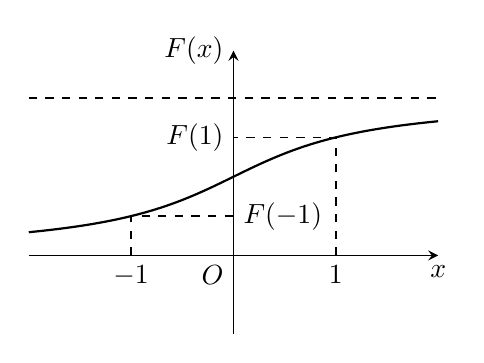
\begin{tikzpicture}[>=stealth,xscale=1.3,yscale=2,semithick]
            \draw[->](-2,0)--(0,0)node[below left]{$O$}--(2,0)node[below]{$x$};
            \draw[->](0,-0.5)--(0,1.3)node[left]{$F(x)$};
            \draw[dashed](-2,1)--(2,1)(1,0)node[below]{$1$}--(1,0.75)--(0,0.75)node[left]{$F(1)$}
            (-1,0)node[below]{$-1$}--(-1,0.25)--(0,0.25)node[right]{$F(-1)$};
            \draw[thick,domain=-2:2,samples=100]plot(\x,{(atan(\x))/180+0.5});
        \end{tikzpicture}
    }
    \subfloat[柯西分布密度函数]{
        \begin{tikzpicture}
            \begin{axis}[
                    axis lines = middle,
                    xlabel=$x$,
                    ylabel={$f(x)$}
                ]
                \addplot[
                    domain=-10:10,
                    samples=100,
                    color=blue,
                ]
                {1/pi/(1+x^2)};
            \end{axis}
        \end{tikzpicture}
    }
    \caption{柯西分布}
\end{figure}

柯西分布的特征:
\begin{description}
    \item[累积函数] $F(x)=\frac{1}{2}+\frac{1}{\pi} \arctan(\mu +\sigma x)$
    \item[矩母函数] 除$t=0$外不存在
    \item[特征函数] $\phi_X(t)=\exp (i \mu t - \sigma |t|)$
    \item[均值] 不存在
    \item[方差] 不存在
\end{description}

\begin{remark}
    此类因极端值概率密度较高而导致均值、方差不存在的分布称为重尾分布。
\end{remark}

\begin{figure*}
    \centering
    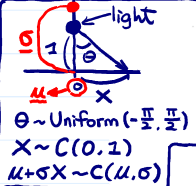
\includegraphics{image/Cauchy_dist.png}
\end{figure*}

\begin{proposition}
    $C(0,1)=t_1$
\end{proposition}

\begin{proposition}
    若随机变量$X,Y \operatorname{i.i.d.} \sim N(0,1)$,则$\frac{X}{Y} \sim C(0,1)$
\end{proposition}

\begin{proof}
    %TODO
\end{proof}

\begin{proposition}
    若随机变量$X \sim C(\mu, \sigma)$,则其线性变换$a,b \in \mathbb{R},aX + b \sim C(a \mu + b,|a| \sigma)$。
\end{proposition}

\begin{proof}
    \[ \phi_{aX + b}(t)=e^{ibt}\phi_X(a t)=\exp (ibt + ia\mu t-\sigma|a t|) \]
\end{proof}

\begin{proposition}
    若独立随机变量$X_1,\cdots ,X_k$满足$ X_i \sim C(\mu_i,\sigma_i)$,则其和$Y=X_1+\cdots +X_k \sim N(\sum_{i=1}^k\mu_i,\sum_{i=1}^k\sigma_i)$
\end{proposition}

\begin{proof}
    \[ \phi_{X_1+\cdots+ X_n} = \prod_{i=1}^n \phi_{X_i}(t)=\exp (it\sum_{i=1}^k\mu_i - |t|\sum_{i=1}^k \sigma_i) \]
\end{proof}

\begin{corollary}
    若随机变量$X_1,\cdots ,X_k \operatorname{i.i.d.} \sim N(\mu,\sigma^2)$,则其平均$\overline{X}=(X_1+\cdots +X_k)/k \sim C(\mu,\sigma)$
\end{corollary}

\begin{remark}
    此处的$\sigma$不代表方差,所以不遵守$\operatorname{Var}(\overline{X})=\frac{\sigma^2}{k}$的关系。
\end{remark}

\section{各分布间关系}

\begin{figure*}[hp]
    \centering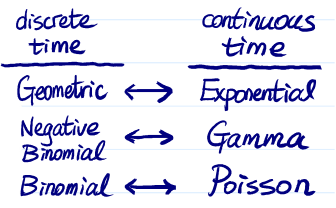
\includegraphics[width=0.95\textwidth]{image/relationship.png}
\end{figure*}

\begin{figure}[hp]
    \centering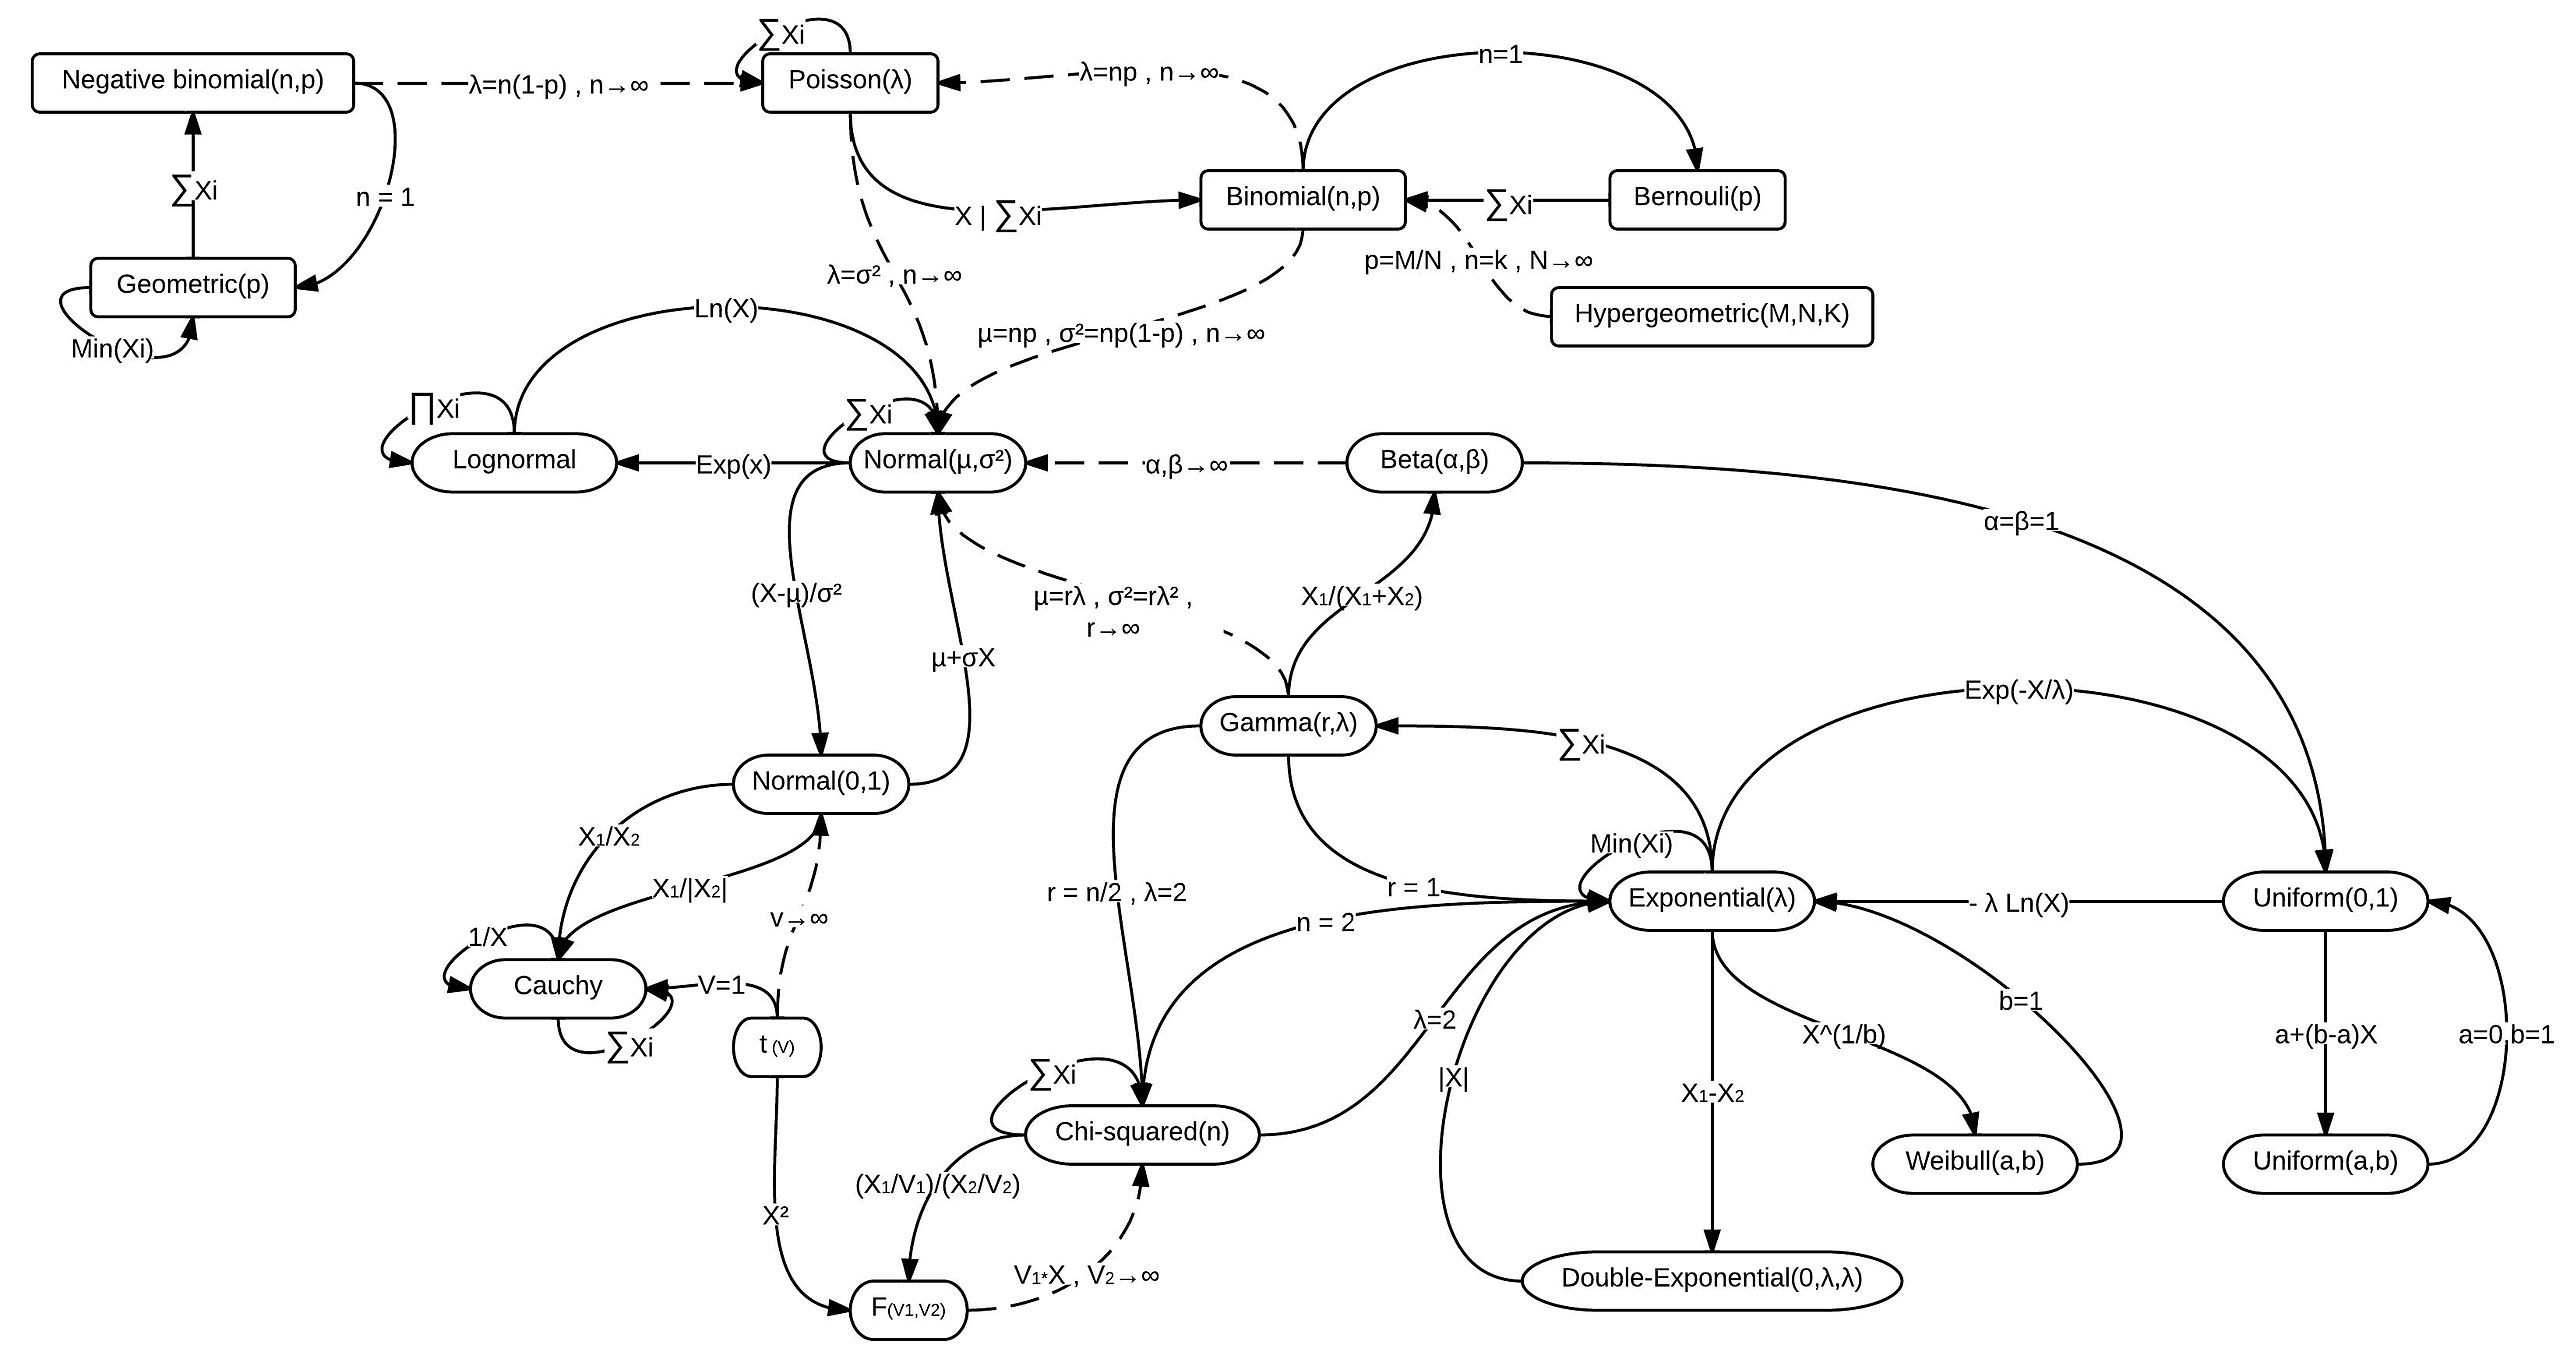
\includegraphics[width=0.95\textwidth]{image/Relationships_among_some_of_univariate_probability_distributions.jpg}
    \caption{各分布间的联系}
    \label{fig:relationship_among_univariate_distributions}
\end{figure}

可参考网站\url{http://www.math.wm.edu/~leemis/chart/UDR/UDR.html}